\documentclass[11pt,a4paper]{article}
\usepackage[margin=2.1cm,top=2.5cm,headheight=26pt]{geometry}
\usepackage{amsmath,amssymb,bm}
\usepackage{siunitx}
\usepackage{booktabs}
\usepackage{graphicx}
\usepackage{tikz}
\usetikzlibrary{arrows.meta,calc,positioning}
\usepackage{enumitem}
\usepackage{float}
\usepackage{xcolor}
\usepackage{fancyhdr}
\usepackage{tcolorbox}
\tcbuselibrary{skins,breakable}
\usepackage[colorlinks=true,linkcolor=blue!60!black,urlcolor=blue!60!black]{hyperref}
\sisetup{per-mode=symbol,detect-all}
\graphicspath{{figs/}}

\definecolor{navy}{RGB}{25,53,73}
\newtcolorbox{keybox}[1]{title={#1},colback=blue!4,colframe=blue!50!black,fonttitle=\bfseries,breakable}
\newtcolorbox{aerobox}[1]{title={#1},colback=orange!5,colframe=orange!60!black,fonttitle=\bfseries,breakable}
\newtcolorbox{sumbox}[1]{title={#1},colback=green!4,colframe=green!40!black,fonttitle=\bfseries,breakable}

% Photograph slot: renders the image if present in figs/, else a dashed placeholder.
% #1 file stem, #2 width fraction, #3 caption, #4 what the picture should show
\newcommand{\photo}[4]{%
  \begin{figure}[H]\centering
  \IfFileExists{figs/#1.jpg}{\includegraphics[width=#2\linewidth]{#1}}{%
  \IfFileExists{figs/#1.png}{\includegraphics[width=#2\linewidth]{#1}}{%
    \begin{tikzpicture}
      \draw[dashed,gray,line width=0.8pt] (0,0) rectangle (#2\linewidth,0.52*#2\linewidth);
      \node[align=center,text width=0.82*#2\linewidth,font=\footnotesize\itshape,gray!70!black]
        at (0.5*#2\linewidth,0.26*#2\linewidth) {PHOTOGRAPH: #4\\[3pt]\ttfamily figs/#1.jpg};
    \end{tikzpicture}}}
  \caption{#3}
  \end{figure}}

\pagestyle{fancy}
\fancyhf{}
\lhead{
\includegraphics[height=0.6cm]{logos/itu_logo_laci.pdf}\ \ UCK 364E Design of Machine Elements}
\rhead{Case Study 3 --- Handout}
\lfoot{\footnotesize Department of Aeronautical Engineering, Istanbul Technical University}
\rfoot{\footnotesize Page \thepage}

\begin{document}

\begin{center}
{\Large\textbf{Case Study: Japan Air Lines Flight 123}}\\[3pt]
{\large\textbf{The fatigue calculation that was right, and killed 520 people anyway}}\\[5pt]
{\small Prof.\ Dr.\ Onur Tunçer \ $\cdot$\ UCK 364E Design of Machine Elements}
\end{center}

\vspace{2pt}\hrule\vspace{6pt}

\noindent\emph{Why you are reading this.} Every other case in this course is a story about a number that came out wrong --- a stress concentration nobody computed, a crack nobody looked for, a test that flattered the design. This one is different, and that is why it is here. After the accident, investigators worked out how many pressurisation cycles the structure could survive. They got \textbf{about 11\,000}. The aircraft flew \textbf{12\,318}. The damage calculation was accurate to roughly ten per cent --- and it saved nobody, because nothing had been built on top of it. No scatter factor. No inspection that could see the critical detail. No second load path. This is the case that tells you what a cumulative-damage number is actually worth.

\photo{ja8119-intact}{0.74}{Boeing 747SR-46 JA8119 in Japan Air Lines service. The SR --- ``Short Range'' --- variant was built for high-frequency domestic sectors, which means it accumulated pressurisation cycles far faster per flight hour than a long-haul 747.}{JA8119 intact, in JAL livery}

\section{What happened}

On the evening of \textbf{12 August 1985}, JAL Flight 123, a Boeing 747SR-46 registered \textbf{JA8119}, left Tokyo Haneda for Osaka Itami with \textbf{524} people aboard. About twelve minutes after take-off, climbing over Sagami Bay, the \textbf{aft pressure bulkhead ruptured}.

What followed is a lesson in load paths rather than in fatigue. The bulkhead separates the pressurised cabin from the unpressurised tail cone. When it failed, cabin air at roughly \SI{60}{kPa} above ambient discharged straight into a structure never designed to hold pressure. The surge blew off most of the \textbf{vertical stabiliser} and severed \textbf{all four hydraulic lines}, which ran together through the same region. The aircraft lost its rudder, its yaw damping, and essentially all flight controls at once.

The crew flew it for a further \textbf{32 minutes} on engine thrust alone, in a phugoid oscillation they could not damp, before it struck a ridge near Mount Takamagahara in Gunma Prefecture at \SI{1565}{m}. \textbf{520 died}; four survived.

\photo{inflight}{0.68}{JA8119 photographed from the ground during the 32 minutes after the failure. Compare the tail with the photograph above: most of the vertical stabiliser is simply gone. The aircraft is still flying --- on thrust alone, with no hydraulics.}{the aircraft in flight with most of the fin missing}

\begin{keybox}{Two separate failures, and only one of them is fatigue}
The bulkhead failed by \emph{fatigue} --- that is the Lecture 4 story, and the subject of this handout. But the accident became unsurvivable because of a \emph{load-path} failure: four hydraulic systems, nominally independent, routed through one place where a single event could cut them all. Redundancy that shares a location is not redundancy. Keep the two lessons separate in your mind; they are both in this course, and they are not the same lesson.
\end{keybox}

\section{The aircraft and its history}

\begin{center}\small
\begin{tabular}{@{}ll@{}}
\toprule
Aircraft & Boeing 747SR-46, JA8119, delivered 1974\\
At the time of the accident & $\approx\SI{25000}{}$ flight hours, $\approx\SI{18800}{}$ cycles\\
Average sector & about \SI{1.3}{hours} per cycle\\
The damaging event & 2 June 1978: heavy landing and tailstrike at Itami,\\
 & operating JAL Flight 115, which \textbf{cracked the aft pressure bulkhead}\\
Cycles at the time of repair & $\approx 6500$\\
Cycles flown after the repair & \textbf{12\,318}\\
Predicted life of the repair & $\approx$ \textbf{11\,000} cycles\\
\bottomrule
\end{tabular}
\end{center}

\medskip
That sector length matters more than it looks. At \SI{1.3}{hours} per cycle, this airframe collected pressurisation cycles perhaps five to seven times faster per flight hour than a long-haul 747 flying ten-hour sectors. The SR variant existed precisely to do that. A maintenance philosophy organised around \emph{hours} is looking at the wrong variable for a pressurised shell --- the same point Aloha 243 makes from the other direction.

\section{The repair}

The 1978 tailstrike cracked the lower half of the aft pressure bulkhead. Boeing sent a team to repair it, and the repair is the whole accident.

The approved method joins the two halves with \textbf{one continuous splice plate}, so that the rivet rows on either side of the seam all carry load \emph{across} the joint. What was actually installed was \textbf{two separate splice plates} on either side of the crack line. The consequence is geometric rather than metallurgical: with the plate cut in two, one of the rivet rows no longer transfers load across the seam at all. The load that should have been shared had to cross through a single effective row.

The investigation assessed the result as retaining about \textbf{70\%} of the fatigue resistance of a correct repair. JAL's post-repair inspection did not catch it, because by then the overlapping plates hid the very detail that was wrong.

\photo{splice-repair}{0.86}{The approved repair (top) and the repair as installed (bottom). In the approved repair a single splice plate carries the joint, and the rivet rows on both sides of it transfer load across the seam. As installed, the plate is in two pieces, and the inboard row no longer crosses the joint.}{the correct and incorrect splice plate arrangements}

\begin{figure}[H]\centering
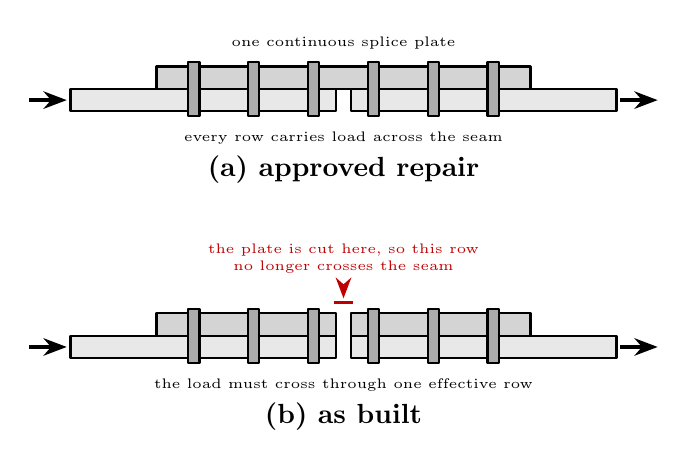
\begin{tikzpicture}[scale=0.95,>=Stealth,font=\scriptsize,line join=round]
\tikzset{web/.style={thick,fill=gray!18},spl/.style={thick,fill=gray!34},
 riv/.style={thick,fill=gray!65},
 bad/.style={red!75!black,line width=1.0pt}}
%--------------- (a) approved: one continuous splice plate ---------------
\begin{scope}
\draw[web] (0,0) rectangle (3.55,0.30);
\draw[web] (3.75,0) rectangle (7.3,0.30);
\draw[spl] (1.15,0.30) rectangle (6.15,0.60);
\foreach \x in {1.65,2.45,3.25,4.05,4.85,5.65}{\draw[riv] (\x-0.075,-0.06) rectangle (\x+0.075,0.66);}
\draw[->,very thick] (-0.55,0.15) -- (-0.05,0.15);
\draw[->,very thick] (7.35,0.15) -- (7.85,0.15);
\node[anchor=south,font=\tiny] at (3.65,0.70) {one continuous splice plate};
\node[anchor=north,font=\tiny] at (3.65,-0.14) {every row carries load across the seam};
\node[anchor=north,font=\bfseries] at (3.65,-0.46) {(a) approved repair};
\end{scope}
%--------------- (b) as built: two plates ---------------
\begin{scope}[yshift=-3.3cm]
\draw[web] (0,0) rectangle (3.55,0.30);
\draw[web] (3.75,0) rectangle (7.3,0.30);
\draw[spl] (1.15,0.30) rectangle (3.55,0.60);
\draw[spl] (3.75,0.30) rectangle (6.15,0.60);
\foreach \x in {1.65,2.45,4.85,5.65}{\draw[riv] (\x-0.075,-0.06) rectangle (\x+0.075,0.66);}
\foreach \x in {3.25,4.05}{\draw[riv] (\x-0.075,-0.06) rectangle (\x+0.075,0.66);}
\draw[bad] (3.52,0.74) -- (3.78,0.74);
\draw[->,bad] (3.65,0.98) -- (3.65,0.80);
\node[bad,anchor=south,font=\tiny,align=center] at (3.65,1.00)
  {the plate is cut here, so this row\\ no longer crosses the seam};
\draw[->,very thick] (-0.55,0.15) -- (-0.05,0.15);
\draw[->,very thick] (7.35,0.15) -- (7.85,0.15);
\node[anchor=north,font=\tiny] at (3.65,-0.14) {the load must cross through one effective row};
\node[anchor=north,font=\bfseries] at (3.65,-0.46) {(b) as built};
\end{scope}
\end{tikzpicture}
\caption{The same two repairs reduced to a load path. The drawing is not to scale; what matters is topological --- cutting the splice plate removes a row from the path across the seam, so the transfer concentrates into what remains.}
\end{figure}

\section{The arithmetic, in the symbols of Lecture 4}

\subsection*{1. Why a factor of 0.7 on stress is not a factor of 0.7 on life}

Finite-life fatigue follows a power law. With $S_a = a N^{b}$ and $b\approx-1/7.7$ for a wrought aluminium alloy, life scales as
\[
N \;\propto\; S_a^{-7.7}.
\]
If a detail change raises the local stress by $1/0.7 = 1.43$, the life falls by $1.43^{7.7}\approx \mathbf{16}$. A 30\% error in a stress estimate is a factor-of-sixteen error in life. This is the single most important number in fatigue design, and it is why ``only 30\% off'' is never a defence.

\subsection*{2. The damage sum}

Taking the investigation's figure of $N_f\approx\SI{11000}{}$ cycles for the as-built repair, and the $n=\SI{12318}{}$ cycles actually flown, Palmgren--Miner gives at the moment of failure
\[
D=\sum\frac{n_i}{N_i}=\frac{12\,318}{11\,000}=\mathbf{1.12}.
\]
Failure at $D=1.12$. For a linear damage rule applied to a real structure, that is an excellent result --- well inside the $D=0.3$ to $D=3$ band in which test data normally fall.

\begin{aerobox}{Read that again, because it is the point of the handout}
The rule worked. The prediction was good. And it was worth nothing, because it existed only in hindsight --- computed \emph{after} the accident, by investigators, from the wreckage. A damage sum is not a safety measure. It is an input to one. What turns it into safety is everything that comes after it: a scatter factor, a retirement or inspection life derived from that factor, an inspection method that can actually see the critical detail, and --- where none of that is reliable --- a second load path.

None of those four existed here. The repair was hidden from inspection by its own plates, the bulkhead was a single load path, and no life limit had been placed on a repair nobody knew was defective.
\end{aerobox}

\subsection*{3. What a scatter factor would have done}

Had the repair been treated as safe-life, with the usual scatter factor of 3 on a predicted life,
\[
N_{\text{safe}}=\frac{11\,000}{3}\approx\mathbf{3\,700}\ \text{cycles}.
\]
The aircraft flew \textbf{3.4 times} that before it failed. Even a crude factor, applied to a number nobody actually had, would have taken the aircraft out of service years early --- or forced an inspection that would have found the cracking while it was still cracking and not yet a rupture.

\section{What the investigation found}

\begin{itemize}[nosep,leftmargin=1.4em]
  \item The probable cause was the \textbf{improper repair} of the aft pressure bulkhead after the 1978 tailstrike, which allowed fatigue cracks to initiate and grow at the rivet line over subsequent pressurisation cycles.
  \item The cracking progressed near the rivet row of the repair until the remaining ligaments could no longer carry cabin pressure, at which point the bulkhead failed over a large area.
  \item The post-repair inspection regime never detected it. The defect was concealed by the repair hardware, and no inspection in the programme was directed at that detail.
  \item The rupture discharged cabin pressure into the unpressurised aft fuselage, destroying the vertical stabiliser and all four hydraulic systems.
\end{itemize}

\photo{fin-damage}{0.95}{Appended Figure 27 of the accident investigation report: damage to the vertical stabiliser, left side. The legend distinguishes wreckage recovered \emph{in the mountains} (cross-hatched), \emph{from the sea} (solid black) and \emph{from beneath the flight path} (dotted). The black regions are the structure that left the aircraft over Sagami Bay --- which is how the investigation established that the fin failed in flight, at the moment of the decompression, and not on impact.}{the investigation report's vertical stabiliser damage diagram}

\section{What changed because of it}

\begin{itemize}[nosep,leftmargin=1.4em]
  \item \textbf{Repairs became design.} A major structural repair is now a certification activity with its own substantiation, its own fatigue assessment, and its own place in the maintenance programme --- not a field activity signed off on completion.
  \item \textbf{Repair Assessment Programmes.} Operators of ageing pressurised aircraft are required to find, document and assess existing repairs for damage tolerance, rather than assume a repair that has not yet failed is sound.
  \item \textbf{Inspectability became a requirement of the repair itself.} A repair that hides the detail it is repairing is not acceptable, because it converts an inspectable structure into an uninspectable one.
  \item \textbf{Hydraulic routing.} Separation of redundant systems in \emph{space}, not merely in schematic, became a sharper requirement.
\end{itemize}

\begin{sumbox}{Five lines to remember}
\begin{enumerate}[nosep]
  \item A cumulative damage sum is an input to a safety argument, not the argument.
  \item Life goes as roughly the seventh power of stress --- a 30\% stress error is a 16$\times$ life error.
  \item A scatter factor exists to cover the things your calculation does not know about. Here, it did not know the repair was wrong.
  \item A repair that conceals the structure it repairs has removed your inspection programme.
  \item Redundant systems routed through one place are one system.
\end{enumerate}
\end{sumbox}

\section{Questions to think about}

\begin{enumerate}[nosep]
  \item The investigation estimated \SI{11000}{} cycles; the aircraft flew \SI{12318}{}. Compute the Miner damage sum at failure. Then state, in one sentence, why this good agreement is not reassuring.
  \item A detail change reduces fatigue resistance to 70\%. Interpret this \emph{two} ways --- as a 30\% reduction in the allowable stress, and as a 30\% reduction in life --- and compute the resulting life ratio in each case using $N\propto S_a^{-7.7}$. Which interpretation is the conservative one to assume when a report does not say?
  \item The airframe flew about \SI{1.3}{hours} per cycle. A long-haul 747 flies about \SI{10}{hours} per cycle. For a pressurised fuselage, by what factor do the two accumulate damage differently \emph{per flight hour}? What does your answer say about maintenance intervals quoted in hours?
  \item Treating \SI{11000}{} cycles as a demonstrated life, compute the safe life for scatter factors of 3 and of 5. For each, state how many years of service at 1\,500 cycles per year this corresponds to.
  \item The bulkhead is a single load path. Sketch two ways you could give a pressure bulkhead a degree of fail-safety, and state for each what the inspection requirement would then be. (Compare your answer with the standby-load-path discussion in class --- which of your two schemes gives an \emph{obvious} partial failure?)
  \item This accident and Aloha 243 both involve fatigue cracking at a riveted row that linked up along the row. List the ways the two cases differ, and say which of the two is better described as widespread fatigue damage.
\end{enumerate}

\section*{Sources and image credits}
\footnotesize
Aircraft Accident Investigation Commission (Japan), report on Boeing 747 SR-100 \textbf{JA8119}, Gunma Prefecture, 12 August 1985. \ FAA, \emph{Lessons Learned from Transport Airplane Accidents} (JAL 123 module). \ Repair assessment and continued-airworthiness requirements: 14 CFR Part 26 and \S25.571; EASA CS-25.571 and AMC 25.571, in the \href{https://www.easa.europa.eu/en/document-library/easy-access-rules/online-publications/easy-access-rules-large-aeroplanes-cs-25}{Easy Access Rules for CS-25}. \ Summary figures for the airframe, the 1978 tailstrike and the repair as reported in the \href{https://en.wikipedia.org/wiki/Japan_Air_Lines_Flight_123}{public account of the accident}; the primary report governs where the two differ.

\medskip
\textbf{Figures.} Figure 1, JA8119 in Japan Air Lines service. Figure 2, the aircraft in flight after the failure. Figure 3, comparison of the approved and as-installed splice arrangements. Figure 5, Appended Figure 27 of the accident investigation report (vertical stabiliser damage diagram, left side). Figure 4 is drawn for this handout. \emph{Verify the licence of each photograph and reproduced figure before distributing beyond the class, and complete the credit line here.} Source files are in the \texttt{figs/} folder beside this \texttt{.tex}; replacing one with a higher-resolution copy of the same subject needs no change to the document.

\end{document}
